\section*{Источники и решения}

\subsubsection*{Трое аборигенов на перекрёстке}

Этот вариант задачи про логика и аборигенов пришёл ко мне от двух матфизиков, Владаса Сидоравичюса и Сени Шлосмана.
Кажется, что «случайный» абориген спутает все карты, однако решение есть.

Сначала надо позаботиться о том, чтобы \emph{второй} спрошенный абориген не был из случайного племени.
Это необходимо, ведь за первый вопрос дорогу не узнать, а если второй абориген случайный, то мы совсем ничего не узнаем.

С другой стороны, этого достаточно, ведь далее можно использовать вопрос с обычным вывертом, типа «А если бы я спросил вас, ведёт ли первая дорога к деревне, вы бы сказали „да“?»

Чтобы достичь этой цели, вам нужно будет спросить аборигена А что-то об аборигенах Б или В, а затем использовать его ответ, чтобы выбрать между Б и В.
Вот работающий вариант: «Верно ли, что Б скажет правду с большей вероятностью, чем В?»

Забавно, что если А ответит «да», то надо спрашивать у В, а если «нет», то у Б!
Ведь если А говорит правду, вы хотите обратиться к тому, кто \emph{меньше} всего склонен говорить правду, то есть к лжецу.
Если же А лжец, то вам нужен \emph{более} правдивый из его спутников, а именно правдолюб.
Конечно же, если А --- «случайный», то вам нет разницы, кого тз остальных выбрать.

В колонках Мартина Гарднера отмечалось, что в исходной задаче с одним аборигеном логик может дойти до деревни даже если забыл, какое из слов на местном языке (предположительно «пиш» и «туш») означает «да» и «нет».
Если желаете развлечься, попытайтесь аналогично изменить описанный выше протокол.

Если случайный абориген выбирает из «да» или «нет», подбрасывая монету в уме, то, конечно же, \emph{одного} вопроса недостаточно.
Однако, если предположить, что он заранее случайно выбирает между правдой и ложью, а затем отвечает логически,
то для этого случая Анупам Джайн из Университета Южной Калифорнии придумал следующий вопрос:
\begin{itemize}
 \item[] \emph{Если я выберу из двух ваших спутников того, чей ответ с наименьшей вероятностью совпадёт с вашим, и спрошу его, ведёт ли первая дорога в деревню, ответит ли он „да“?}
\end{itemize}
Утверждается, что если ответ «нет», то первая дорога --- правильная, в противном случае --- вторая.

Ключевой случай: этот вопрос задан случайному отвечающему.
Если случайный абориген решит солгать, то ответ правдолюба на вопрос будет наименее вероятно совпадать с его ответом.
Правдолюб скажет «да», и так как случайный отвечающий решил солгать, он скажет противоположное и, таким образом, ответит «нет».

Если случайный отвечающий решил сказать правду, то ответ правдолюба будет наименее вероятно совпадать с его ответом.
Лжец скажет «нет», и так как случайный отвечающий решил сказать правду, он опять скажет «нет».

Если логик обращается к правдолюбу, то ответ лжеца наименее вероятно совпадёт с его ответом, и он скажет то, что сказал бы лжец: «нет».

Точно так же, если вторая дорога правильная, все ответы будут «да».

\begin{addedbytheeditors}
Есть более сложный вариант этой задачи, предложенной американским философом и логиком Джорджем Булосом в итальянской газете «la Repubblica» в 1992 году%
\footnote{Булос указывает логика Рэймонда Смаллиана как автора задачи (похожие сюжеты есть в книге~\cite{52}) и Джона Маккарти как человека, придумавшего более сложную формулировку из-за неясных трактовок «da» и «ja».
Обсуждение этого, более сложного варианта задачи, см. в
%\href{https://en.wikipedia.org/wiki/The_Hardest_Logic_Puzzle_Ever}{https://en.wikipedia.org/wiki/The_Hardest_Logic_Puzzle_Ever}.
}:

Есть три бога: A, B и C, которые являются богами истины, лжи и случая в произвольном порядке.
Бог истины всегда говорит правду, бог лжи~--- всегда обманывает, бог случая либо говорит правду, либо лжёт, что определяется случайным образом. Требуется определить богов, задав 3 вопроса, на которые можно ответить <<да>> или <<нет>>. Каждый вопрос задаётся только одному богу, но можно задавать одному богу более одного вопроса. Боги понимают язык, но отвечают на своём языке, в котором есть 2 слова <<da>> и <<ja>>, причём неизвестно, какое слово обозначает <<да>>, а какое <<нет>>.\pr
\end{addedbytheeditors}

\subsubsection*{Новая встреча с тремя окружностями}

Эту задачу иногда называют «окружностями Монжа».

На сайте Cut-the-Knot \cite{cut-the-knot} следующее доказательство приписывается Натану Боулеру из Тринити-колледжа в Кембридже.
Оно использует конусы, построенные на окружностях вместо сфер.
Обозначим их через $C_1$, $C_2$ и $C_3$; мы предполагаем, что это прямые конусы, то есть с углом $90\degree$ при вершине.
(На самом деле, достаточно, чтобы углы при их вершинах были одинаковы.)
Каждая пара конусов определяет две (внешние) касательные плоскости, скажем, $P_1$ и $Q_1$ (для конусов $C_2$ и $C_3$), $P_2$ и $Q_2$ (для конусов $C_1$ и $C_3$), и, наконец, $P_3$ и $Q_3$ (для конусов $C_1$ и $C_2$).

Каждая пара плоскостей $P_i$, $Q_i$ пересекается по прямой $L_i$, которая проходит через вершины конусов, а также через точку, где соответствующие касательные пересекаются.
Таким образом, прямые $L_1$ и $L_2$ проходят через вершину $C_3$,
прямые $L_1$ и $L_3$ через вершину $C_2$,
а $L_2$ и $L_3$ через вершину $C_1$.
Следовательно, эти три прямые лежат в плоскости, определённой тремя вершинами конусов. Пересечение этой плоскости с исходной плоскостью окружностей и есть та самая прямая, проходящая через три центра перспективы --- победа!

\begin{addedbytheeditors}
Вместо конусов можно было построить сферы, касающиеся данной плоскости и радиусами, равными радиусам данных окружностей. К ним можно провести вторую касательную плоскость, которая в пересечении с первой даст прямую, на которой лежат три фокуса.

Есть ещё одна идея, которая позволяет исправить решение, данное в комментарии к условию задачи\footnote{В.Протасов Выход в пространство-2 (продолжение). Квант №1 2018.}.
Во-первых, можно считать, что центры
шаров не лежат на одной прямой (если
лежат, то утверждение очевидно). Во-вторых, если одновременно уменьшить радиусы шаров в $N$ раз, оставив на месте их
центры, положение фокусов не изменится. Для достаточно большого $N$ каждая сфера окажется вне конуса, описанного около  пары других сфер. Значит, можно будет найти пару плоскостей, касающихся уменьшенных сфер. 
\pr
\end{addedbytheeditors}

\subsubsection*{Самоубийцы Точкинска}

Эта головоломка про знания о знаниях удивляет своей общностью.
Она досталась мне от Ника Рейнголда из AT\&T Labs.
Различные частные случаи (иногда с наводящими ужас формулировками%
\footnote{Есть вариант про казни неверных жён.\pr}%
) известны на протяжении многих десятилетий.
Многим из вас наверняка известен вариант, когда у всех точки синие, а приезжий сказал: «Есть хотя бы одна синяя точка».

То есть, что им ни скажешь, --- будет катастрофа, и это впечатляет.
Но, ещё удивительней, что все обречены даже \emph{если каждый видит, что приезжий соврал}. 
Мы это скоро докажем, но сначала рассмотрим простой частный случай, показывающий, как это работает.

Предположим, что в Точкинске живут всего три жителя, и у всех на лбу синие точки, а приезжий сказал им, что все точки красные.
Конечно же все видят, что это не так.
Однако первый из них думает следующее: предположим, что моя точка красная; тогда второй житель видит мою красную точку и задаётся вопросом, видит ли третий житель две красные точки?

«Если так» --- думает второй, --- «то третий житель поверит приезжему и совершит самоубийство этой же ночью, несмотря на то, что у него точка синяя».

Если же этого не произошло, то второй житель правильно заключит, что третий увидел только одну красную точку, и совершит самоубийство во вторую ночь.
Поскольку ни одно из этих событий не происходит, первый житель заключает, что второй не увидел красной точки.
Он заключает, что его точка синяя, и прощается с жизнью на третью ночь.

Для доказательства общего случая введём некоторые обозначения.
Пусть $S\subset\{0,1,\dots,n\}$ --- множество чисел $x$ с таким свойством: \emph{если у $n$ точкинцев $x$ синих точек, то утверждение приезжего верно}.
По предположению, $S$ --- собственное подмножество; то есть $S$ и его дополнение непусты.
Пусть $b$ --- число синих точек на самом деле;
$b$ может принадлежать $S$, а может и не принадлежать.

Обозначим через $B_i$ множество возможных чисел синих точек, с точки зрения $i$-того точкинца.
Если $b_i$ --- число синих точек, которое он видит на других, то до заявления приезжего, $B_i=\{b_i,b_i\z+1\}$.

Если в какой-то момент $B_i$ сокращается до одного значения, то $i$-й точкинец обречён.
Это произойдёт в первую же ночь в случае, если  $|B_i\z\cap S|=1$, но это произойдёт и на следующую ночь после любого самоубийства.
Действительно, все точкинцы с одинаковым цветом точек ведут себя одинаково, ведь они все видят одинаковое число точек каждого цвета.
Таким образом, если какой-то точкинец видит, что кто-то совершил самоубийство, то (справедливо) считает, что цвет точки этого человека отличается от его собственного. 
Следовательно, он знает свой собственный цвет и обречён.

Для заданных $S$ и $b$ обозначим через $d(b)$ наименьшее число шагов (увеличений или уменьшений на $1$), необходимое для того, чтобы попасть из $b$ за пределы $S$ или внутрь $S$.
Другими словами, $d(b)$ это наименьшее $k$, такое что $b+k$ или $b-k$ находится в $\{0, 1, \dots, n\}$, но не в $S$ (если $b$ не в  $S$) или в $S$ (если $b$ в $S$).

Например, если $n=10$ и 
$S=\{0,1,2,9,10\}$, то 
$d(0)=3$, 
$d(1)=2$, 
$d(2)=d(3)=1$, 
$d(4)=2$, 
$d(5)=d(6)=3$, 
$d(7)=2$, 
$d(8)=d(9)=1$ и
$d(10)=2$.

Как уже отмечалось, если $d(b)=1$, то самоубийства произойдут уже в первую ночь.
Теперь сделаем более общее утверждение: \emph{первые самоубийства произойдут именно в $d(b)$-ю ночь}.

Доказательство ведётся индукцией по $d(b)$.
Предположим, что это верно при $d(b)<t$, а теперь пусть $d(b)=t>1$.
После $(t-1)$-й ночи, поскольку самоубийств ещё не было, все знают, что $d(b)\ge t$.
Однако, если $d(b)=t$, то $d(b-1)$ либо $d(b+1)$ равно $t-1$.
В первом случае синеточкенцы, которые знают, что синих точек $b$ (то, что на самом деле) или $b-1$, 
могут исключить случай $b-1$, и им конец.
Во втором случае красноточкинцы могут исключить $b+1$, и им придётся покончить с собой.
Наконец, если $d(b-1)\z=d(b+1)=t-1$, то никто не переживёт эту ночь.

Поскольку $d(b) \le n$, то к $n$-й ночи все погибнут.
Также можно увидеть, что они продержатся столько времени только в четырёх крайних случаях:
если $b=0$ и $S=\{n\}$ или $\{0,1,\dots,n-1\}$,
а также если $b=n$ и $S=\{0\}$ или $\{1,2,\dots,n\}$.
Иначе говоря, время выживания максимально, если приезжий либо делает наименее информативное верное заявление,
либо высказывает самую безумную ложь.
Также стоит отметить, что определение $d(b)$ не различает $S$ и его дополнение --- точкинцы будут вести себя точно так же независимо от того, скажет ли приезжий «$X$» или «Не $X$».

Можно было бы задаться вопросом, а могут ли точкинцы, зная, что к ним едет кто-то, кто может нарушить (явно оправданное!) правило молчания о цвете точек, организовать для себя какую-то защиту.
Например, все, кто знает, что приезжий соврал, поднимаются и говорят об этом.
К сожалению, немного поразмыслив, можно прийти к выводу, что ни эта, ни какая-либо другая стратегия не спасёт город.

Да, жизнь точкинцев висит на волоске.
Но как ни странно, это и может их спасти.
Стив Бэббидж, менеджер и криптограф из компании Vodafone, указал на то, что при определённых обстоятельствах некоторые точкинцы смогут пережить вторжение приезжего, если подумают, что чьё-то самоубийство было вызвано не знанием цвета, а тем, что тот не выдержал жизни в их смехотворной среде.

\subsubsection*{Заражённые кубы}

То, что изначально \emph{нужно} хотя бы $n^{d-1}$ заражённых единичных кубов (для краткости \emph{участков}), доказывается прямым обобщением двумерного случая, в котором, как мы знаем, периметр заражённой области не увеличивается.
Вместо периметра следует взять $(d\z-1)$-мерную площадь поверхности заражённой области.
Когда новый участок заражается, к этой поверхности добавляется не более чем $d$ его граней,
и в то же время по крайней мере $d$ граней удаляются (те, что отделяют новый участок от заражённых соседей).
Таким образом, площадь поверхности не увеличивается.
В самом конце, она равна площади поверхности большого куба, что составляет $2d \times n^{d-1}$.
Поскольку каждый участок имеет $2d$ граней единичной площади,
начальная площадь поверхности не может превышать $k \times 2d$,
где $k$ --- число изначально заражённых участков.
Отсюда $k\geqslant n^{d-1}$.

Однако на этот раз выбрать начальные $n^{d-1}$ заражённых участков совсем не просто.
Мэтт Кук и Эрик Уинфри из Калтеха нашли способ, который должен срабатывать, но не смогли этого доказать;
впоследствии их коллега Лен Шульман придумал замечательное доказательство, приведённое ниже (присланное мне Эриком).

Начнём с построения Мэтта и Эрика.
Обозначим участки векторами $(x_1 , x_2 , \dots , x_d )$, где $x_i \in \{1, 2, \dots , n\}$, так что два участка соседствуют, 
если все их координаты, кроме одной, одинаковы, а эта одна различается на $1$.

Возьмём любое целое число $k$ и заразим все участки, для которых $\sum_i x_i \equiv k\pmod n$.
Эти участки образуют \emph{диагональное подпространство}, оно разбивается на несколько кусков.
Они всё заражают, но странным образом и очень по-разному при разных $k$.
Часто кажется, что просто повезло из-за нескольких совпадений. 
Картина сильно отличается от двумерной!

В доказательстве, что это множество годится, Шульман использовал следующую игру;
в ней сила, препятствующая заражению, передана демону-противнику, который мешает заражающему игроку.
Выберем $k$ и начнём с заражённых участков, описанных выше.

Сначала демон помещает вас на участок $x = (x_1, \dots,x_d )$.
Далее он выбирает координату $i$.
У вас есть право переместится либо вперёд, либо назад вдоль $i$-й координаты (если $x_i=1$ или $x_i=n$, то выбора нет).
Вы выигрываете, если сможете достичь некоторой точки $x$, из диагонального подпространства $\sum_i x_i \equiv k\pmod n$;
демон выигрывает, если сможет заставить вас бесконечно блуждать.

Утверждается, что если у вас есть стратегия, которая гарантирует победу против демона, то заразится весь большой куб.

Прежде чем доказывать, уточним утверждение: если можно выиграть, начав с $x$, то $x$ заразится.
Действительно, демон может выбрать любое из $d$ направлений,
и победная стратегия срабатывает при каждом выборе.
Это означает, что с вашей стратегией можно победить, начав с любого из $d$ соседей $x$, к которым вы собирались переместиться.
По индукции (по числу шагов до победы), все эти $d$ соседей $x$ заразятся, а значит, заразится и $x$.
За базу индукции возьмём случай, с начальным участком $x$ из диагонального подпространства --- в этом случае он уже заражён.

Осталось описать выигрышную стратегию.
Далее следует то, что Шульман называл \emph{алгоритмом телеги}.
Для любого участка $x$ обозначим через $x^*$ значение $-k + \tfrac12 + \sum_i x_i \pmod n$.
Если демон выбрал $i$-ю координату, то следует уменьшить $x_i$ если $x_i > x^*$ (таким образом, $x^*$ также уменьшается, хотя, возможно, и прыгнет с $\tfrac12$ на $n - \tfrac12$).
Если же, $x_i < x^*$, то надо увеличить $x_i$, чтобы значение $x^*$ также увеличилось, или возможно, прыгнуло с $n - \tfrac12$ на $\tfrac12$.
Но постойте --- если вы попали на участок с $x^* = \tfrac12$, то победа ваша!

Отсюда следует, что ход, предписанный алгоритмом, всегда допустим:
нет нужды ходить на участок с $x_i = 0$ или $x_i = n + 1$, до победы.

Теперь мы утверждаем, что демон не может заставить вас зациклиться.
Предположим противное, то есть $x$ циклически повторяется.
Пусть $I$ --- множество индексов, выбранных демоном бесконечное число раз.
Можно считать, что вы уже прошли сколько шагов, что уже ни один индекс, не принадлежащий $I$, больше выбран не будет.
Пусть $y$ будет самым большим значением $x_j$, когда-либо встречавшимся для любого $j \in I$.
Пусть $J$ --- множество индексов в $I$, которые в данный момент имеют это максимальное значение $y$.

Если когда-либо случится, что $x^* > y$, то вы будете увеличивать его на каждом шаге, увеличивая $x^*$, пока он не прыгнет в $\tfrac12$, принеся вам победу.
Следовательно, $x^*$ всегда меньше $y$.
Но тогда, когда демон выбирает $j \in J$, $x_j$ должен уменьшаться до $y - 1$.
В результате $J$ в конечном итоге исчезнет, оставив вас навсегда с меньшим максимальным значением $y$.
А это не может продолжаться вечно --- противоречие.

Отсюда следует, что алгоритм телеги позволяет выигрывать, независимо от того, куда вас высадил демон или как он вас ограничивал.
Существование выигрышной стратегии означает, что заразится весь большой куб --- ура!

\subsubsection*{Шляпы и бесконечность}

Оба ответа --- «Да, стратегия существует» и «Нет, её нет» --- оказываются верными!
Но разве такое возможно?

По моим данным, эта прекрасная загадка была придумана совместно Ювалем Габаем и Майклом О'Коннором (в то время аспирантами Корнельского университета).
Однако решение косвенно содержалось в работе Фреда Гальвина из Канзасского университета.
Кристофер Хардин (Колледж Смита) и Алан Д. Тейлор (Колледж Юнион) затем включили её в статью для American Mathematical Monthly \cite{36}.
Стэн Уэгон предложил её как задачу недели в Маккалестерском колледже.
Дополнительные интересные наблюдения об этой и следующей задаче были сделаны Харви Фридманом (Огайо Стейт), Хендриком Ленстрой (Университет Лейдена) и Джо Булером (Рид Колледж).
Последний из них, а также (независимо) Мэтт Бейкер из Технологического института Джорджии, рассказали мне о ней.
Всё это только небольшая часть истории.
Простите меня, если пропустил ваше имя!

Сначала посмотрим, а что если только конечное число заключённых получат красные шляпы.
Тогда все заключённые это увидят, и если они заранее договорились об этом, все скажут «синий» --- и, конечно же, только конечное число ошибётся.

Та же схема применима, и если только конечное число шляп будут синими или, например, если только конечное число шляп с нечётными номерами будут красными, а конечное число шляп с чётными номерами будут синими.
Можно пойти ещё дальше: если последовательность шляп \emph{периодична} с какого-то места, то все могут угадать цвет, как если бы последовательность была периодичной с самого начала.

Другими словами, последовательность цветов шляп можно считать двоичной записью некоторого вещественного числа $r$ из интервала $[0,1]$, считая (скажем) синий как 1, а красный как 0.
\emph{С какого-то места периодична} означает, что с какого-то момента некоторое слово из нулей и единиц в ней бесконечно повторяется;
это означает, что $r$ рационально.
Например, последовательность $100101001010101010\dots$, где $01$ бесконечно повторяется, является таким числом; в этом случае число равно дроби $7/12$.
Если так произошло, то каждый заключённый с нечётным номером может сказать <<синий>>, а каждый с чётным номером --- <<красный>>, и все, кроме номеров $3$, $4$, $5$, $6$ и $7$, окажутся правы.

Таким образом, заключённые спасутся, если $r$ рационально.
Однако нет нужды ограничивать стратегию рациональными числами.
Возможно, последовательность будет отличаться лишь в конечном числе мест от двоичного представления $\pi$, в таком случае заключённые могут согласиться угадывать, как если бы шляпы представляли собой точно $\pi$.

На самом деле заключённым надо разделить все возможные последовательности шляп на такие \emph{классы}, что в каждом классе две последовательности отличаются только в конечном числе мест.
Затем заключённые заранее договариваются о представителе из каждого класса, то есть о каком-то конкретном члене класса.
Если они видят последовательность из этого класса, то каждый угадывает, как если бы фактическая последовательность была равна согласованному представителю.

Более математически, мы говорим, что две последовательности \emph{соседние}, если они отличаются только в конечном числе мест.
Заметим, что
(1) любое $r$ --- сосед самого себя;
(2) если $r$ --- сосед $s$, то $s$ --- сосед $r$; и
(3) если $r$ --- сосед $s$, и $s$ --- сосед $t$, то и $r$ --- сосед $t$.
Это означает, что соседство является тем, что математики называют \emph{отношением эквивалентности}.
В свою очередь это означает, что существует такое разбиение множества всех последовательностей шляп на классы, что в каждом классе любые две последовательности будут соседними, а любые две последовательности из разных классов соседними не будут.

Пока всё чисто, но сейчас появится трудность.
Большинство этих классов не будут обладать естественным представителем (как например $\pi$),
и заключённым придётся как-то договориться о представителе в каждом классе.
Утверждение о том, что это в принципе возможно сделать, называется \emph{аксиомой выбора}.
Если принять аксиому выбора, то заключённые смогут ей воспользоваться, чтобы выбрать по представителю из каждого класса.
Затем, увидав шляпы, заключённые поймут, к какому классу принадлежит последовательность шляп (для этого достаточно смотреть только на шляпы заключённых с более высокими номерами, чем их собственные).
Затем они все угадывают, что их собственный цвет шляпы такой, как это предсказано согласованным представителем класса, и допускают только конечное число ошибок --- дело сделано!

Но считать ли аксиому выбора верной?
Большинство активно работающих математиков предполагают, что да.
Однако известно, что если основные аксиомы с аксиомой выбора образуют непротиворечивую систему, то нет противоречия и с отрицанием аксиомы выбора.
Так что так же справедливо предположить, что аксиома выбора не выполняется, как и предположить, что она выполняется.

А если аксиома выбора не выполняется, то заключённые окажутся в трудном положении.
Упомянутые выше Хардин и Тейлор, и независимо Харви Фридман, показали, что если принять отрицание аксиомы выбора, у заключённых нет выигрышной стратегии.
И даже хуже: любая стратегия потерпит неудачу, если только, в определённом смысле, который можно сделать математически точным, заключённые не будут невероятно удачливы.
Так что, если есть опасность стать заключённым, то лучше принять аксиому выбора (и взять её с собой).

А сами вы верите в аксиому выбора?
Подумайте: множество возможных выигрышных стратегий для нашего предполагаемого решения является произведением всех вышеобсуждаемых классов эквивалентности; если нет решения, это означает, что произведение бесконечного числа непустых (да ещё и бесконечных) множеств пусто.
С другой стороны, знаменитый парадокс Банаха --- Тарского утверждает, что, используя аксиому выбора, можно разрезать шар на пять частей и собрать из них два шара, идентичных исходному!

У меня такой вывод: хотя ни аксиому выбора, ни её отрицание нельзя опровергнуть, любую из них можно сделать смешной.

%\begin{addedbytheeditors}
%\textbf{Редакторам:} Заменил «без аксиомы выбора» на «с её отрицанием», иначе фраза бессмысленна. 
%\end{addedbytheeditors}
% 

\subsubsection*{Все правы или все неправы}

Если вы разобрались с решением предыдущей головоломки (с аксиомой выбора), то и здесь не должно быть проблем.
Во-первых, заключённые соглашаются, как и раньше, на представителя из каждого класса эквивалентности.
Кроме того, они соглашаются, что будут угадывать цвет своих шляп исходя из предположения, что число позиций, в которых последовательность шляп не совпадает с выбранным представителем, чётно.
Как и в случае конечного числа, если это число чётно, то все заключённые будут правы; в противном случае --- все неправы.

Примечательно, что алгебраисты обычно решают эту задачу следующим образом.
Отождествим цвета шляп с множеством $\{0, 1\}$, --- то есть, как и раньше, 
будем думать, что это элементы группы $\mathbb{Z}_2$.
Сумма $\Sigma$ из бесконечного числа копий $\mathbb{Z}_2$ является множеством всех последовательностей из 0 и 1, в которых только конечное число единиц (синие шляпы).
Существует естественный гомоморфизм (отображение) из $\Sigma$ в $\mathbb{Z}_2$, который даёт 0, если число единиц чётно, и 1, если нечётно.
Стандартная теорема о расширении позволяет нам расширить этот гомоморфизм на произведение $\mathbb{Z}_2$, которое является множеством всех последовательностей $\{0, 1\}$.
Затем заключённые соглашаются угадывать, предполагая, что значение этого гомоморфизма равно (скажем) 0.

Конечно, в \emph{доказательстве} теоремы о расширении нужна аксиома выбора, поэтому это доказательство на самом деле ничем не отличается от других.

Означает ли это, что для версии с «все правы» или «все неправы» бесконечной задачи о шляпах также требуется аксиома выбора?
Я так думал, пока Тина Кэрролл (студентка-математик в Технологическом институте Джорджии) не показала мне решение, которое \emph{гораздо} проще и не требует аксиомы выбора или какой-либо математики вообще.

Каждый говорит «зелёный»!!

\begin{addedbytheeditors}
Про гомоморфизм $\mathbb{Z}_2^\infty\to \mathbb{Z}_2$ можно думать, как про обобщённую сумму бесконечной последовательности элементов из $\mathbb{Z}_2$.
Поэтому второе решение --- это по сути спасение рассуждения с чётностью числа красных шляп, прекрасно работающего в конечном варианте задачи.
Про этот гомеоморфизм можно думать уймой способов, например как об ультрапределе суммы первых $n$ членов последовательности по неглавному ультрафильтру.
Можно действовать и более геометрически, через выбор точки в чех-стоуновской компактификации натуральных чисел.\pr
\end{addedbytheeditors}


\subsubsection*{Цифры на лбах}

Эта головоломка пришла ко мне независимо от нескольких людей, включая Ногу Алона из Тель-Авивского университета.
Сам Нога многократно показывал, что во многих задачах полезно ввести вероятность, даже если в формулировке её не было.
В нашей задаче, если предположить, что числа на лбах выбираются независимо и равномерно случайным образом, то каждый заключённый угадает правильно с вероятностью $\tfrac{1}{n}$ независимо от того, что именно он скажет.

Положим, что заключённые пронумерованы от $0$ до $n-1$.
Мы хотим, чтобы вероятность того, что какой-то заключённый угадает правильно, была равна $1$.
Значит нам нужно, чтобы $n$ событий типа \emph{«$k$-й заключённый угадывал правильно»} были бы взаимоисключающими.
Другими словами, ни одно из них не может произойти одновременно с другим.
В противном случае вероятность хотя бы одного успешного исхода была бы строго меньше суммы $\tfrac1n + \tfrac1n + \dots + \tfrac1n = 1$.

Для этого следует разделить всевозможные расстановки чисел на $n$ равновероятных сценариев, а затем потребовать, чтобы заключённые основывали свою догадку на разных сценариях.
Эта идея приводит к следующему простому решению.
Если $s$ --- сумма чисел на лбах по модулю $n$, то пусть $k$-й заключённый считает, что $s = k$.
Другими словами, он считает, что его собственное число равно $k$ минус сумма оставшихся чисел по модулю~$n$.

В этом случае $s$-й заключенный будет прав, а все остальные --- нет.

\subsubsection*{Заключённый дальтоник}

Из-за Майкла со Шреком заключённые не смогут реализовать схему из предыдущего решения.
Но это само по себе не означает, что другого решения не существует.

Тем не менее мы видели, что успешная схема должна предотвратить возможность угадывания правильного числа одновременно двумя заключёнными, и это, возможно, грозит Шреку неприятностями.

Предположим, что \emph{существует} успешная схема; можно считать, что Шрек знает,  \emph{что} в точности будет делать Майкл,
ведь он видит каждое число, которое видно Майклу.
Поскольку он видит число Майкла, то он может с некоторой вероятностью ($\tfrac1n$) знать, что Майкл угадает правильно.

В этом случае Шрек должен угадать неправильно, но поскольку он не знает своего собственного числа, у него нет возможности это сделать наверняка.
(Выстрелить в воздух, например, назвав $n + 1$, не сработает, ведь тогда сумма вероятностей успеха не достигнет 1.)
Значит заключённые потерпят неудачу с положительной вероятностью.

\subsubsection*{Числа со шляпами}

Эту головоломку мне прислала Николь Имморлика, постдок из Microsoft Research.
Её формулировка (и решение) содержится в статье шести авторов \cite{1}, где она используется в явной конструкции для высокодоходных детерминированных аукционов.

Заключённые могут гарантированно выиграть независимо от распределения чисел.
Прежде чем на лбах появятся числа, они выберут порядок, то есть пронумеруют себя от $1$ до $n$ (скажем, по алфавиту).
Когда все увидят числа, $i$-й заключённый (для каждого $i$) заводит новую нумерацию остальных числами от $1$ до $i - 1$ и от $i + 1$ до $n$, в порядке чисел на их лбах.
Далее он вычисляет, сколько транспозиций старых номеров требуется, чтобы перевести их на место новых номеров.

Предположим, что позже этот $i$-й заключённый узнал своё число, и оказалось, что оно стоит на $j$-м месте после упорядочивания по возрастанию.
Тогда ему придётся сделать ещё $|i - j|$ транспозиций, чтобы завершить перестановку $\sigma$ от всех $n$ старых номеров к $n$ новым номерам.
Действительно, $i$ и $j$ следует поменять местами, а числа между ними нужно сдвинуть вверх или вниз на одну позицию.

Например, предположим, что $n = 4$ и $3$-й заключённый видит на лбах $1$-го, $2$-го и $4$-го числа $2\pi$, $\pi$ и $4\pi$ соответственно.
Тогда он присваивает им новые номера 2, 1 и 4.
Чтобы получить эти номера из старых 1, 2 и 4, надо поменять местами 2 и 1 --- одна транспозиция.
Если он ставит себя на 3-е место, то получает перестановку $1234 \to  2134$.
Его собственное число может быть, скажем, $\pi/2$, и значит он должен был быть первым, а не третьим.
Чтобы получить правильную перестановку  $\sigma  = 1234 \to  3214$, ему надо поменять местами 3 и 1, а затем 2 и 3, то есть нужны ещё две транспозиции.
Конечно же число могло оказаться другим --- мы привели этот последний шаг, чтобы помочь разобраться в последующем  рассуждении.

Допустим, что $\sigma$ --- чётная перестановка, то есть она реализуется чётным числом транспозиций.
Тогда исходная перестановка $i$-го заключённого будет чётной, если $|i - j|$ чётно, и нечётной в противном случае.
Конечно, если $\sigma$ нечётна (как в примере), то справедливо обратное.

Итак, $i$-му заключённому следует выбрать красную шляпу, если он насчитает чётное число транспозиций (в его перестановке остальных $n - 1$ чисел) и его собственный старый номер $i$ чётен, или же если он насчитает нечётное число транспозиций, и $i$ нечётно.
В противном случае он выбирает синюю.
В приведённом примере $i$ нечётно, и $3$-й заключённый сделал нечётное число (одну) транспозицию, поэтому он выберет красную шляпу.

Если перестановка $\sigma$ оказалась чётной, то этот выбор означает, что заключённый $i$ будет выбирать красную шляпу только тогда, когда $i$ и $|i - j|$ оба чётны или когда $i$ и $|i - j|$ оба нечётны --- другими словами, когда $j$ чётно.
Таким образом, в новом порядке каждый заключённый с чётным номером будет носить красную шляпу, а каждый с нечётным --- синюю.

Если же $\sigma$ нечётна (как в примере), то в новом порядке красные шляпы будут надеты на заключённых с нечётными номерами, и в любом случае они победят.

\subsubsection*{Кирпичная стенка}

Вопрос о том, как уложить $n$ кирпичей, максимизируя их выступ за край стола, был поставлен в 1923 году Дж. Г. Коффином \cite{12}.
Однако другие эквивалентные формулировки известны с 1850 года.
Благодаря Мартину Гарднеру этот вопрос стал очень известным, и его используют по всему миру для первого знакомства с гармоническим рядом.

Забавно, но несмотря на широко распространённое мнение об обратном, знаменитая \emph{гармоническая стопка} (см. рис. \ref{pic:kirpich1}) далека от оптимального решения (иногда, впрочем, в условия добавляют ограничение одного кирпича на уровень).
Более того, часто отмечается, что до начала постройки надо решить, какого выступа мы хотим добиться --- но и это тоже неверно.

\begin{figure}[ht!]
\centering
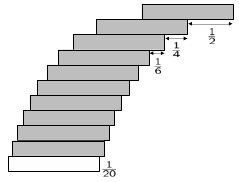
\includegraphics[scale=1]{pics/kirpich1}
\caption{Десятикирпичная гармоническая стопка.}
\label{pic:kirpich1}
\end{figure}

Чтобы получить гармоническую башню, заметим что верхний кирпич не может выступать за  кирпич под ним больше, чем на $1/2$ (при единичной длине кирпича).
В этом случае центр тяжести двух верхних кирпичей находится на $1/4$ левее края нижнего кирпича, поэтому второй сверху кирпич не может выступать за следующим под ним, больше, чем на $1/4$.
Продолжая таким образом, $k$-й сверху кирпич, выступает на $\tfrac1{2k}$ над $(k + 1)$-ым, а значит общий выступ составит 
\[\tfrac12+\tfrac14+\dots+\tfrac1{2k}=\tfrac12(1+\tfrac12+\dots+\tfrac1k)=H_n/2,\]
где $H_n$ --- $n$-я частичная сумма гармонического ряда, она растёт как натуральный логарифм~$n$.

Поскольку гармонический ряд расходится, можно прийти к (верному) выводу, что если кирпичей достаточно, то можно добиться произвольно большого выступа.
Если строить башню таким образом, то придётся решить заранее, какой выступ нам нужен --- он ограничен положением самого нижнего кирпича.

\begin{figure}[htb!]
\centering
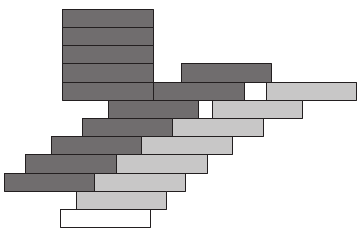
\includegraphics[scale=1]{pics/kirpich2}
\caption{Максимальный выступ для 19-и кирпичей.}
\label{pic:kirpich2}
\end{figure}

Однако можно добиться большего, если использовать несколько кирпичей в качестве противовеса.
В декабре 2005 года Дж. Ф. Холл \cite{35} отметил, что общий выступ можно увеличить примерно вдвое (то есть, сделать его около $\ln n$) используя стопку кирпичей, в которой каждый выступает над предыдущим, а противовесом к ним служат дополнительные кирпичи. %??? она не ``cover article''
На самом деле, вплоть до 19 кирпичей такие стенки дают максимальный выступ; см. рис. \ref{pic:kirpich2} для случая $n = 19$.
Однако Холл неверно заключил, что его стенки (называемые хребетными из-за того, что кирпичи, поддерживающие самый крайний кирпич, образуют стопку с одним кирпичом на уровень) оптимальны в общем случае.

\begin{figure}[htb!]
\centering
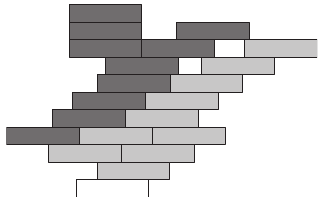
\includegraphics[scale=1]{pics/kirpich3}
\caption{Максимальный выступ для 20-и кирпичей.}
\label{pic:kirpich3}
\end{figure}

\begin{figure}[htb!]
\centering
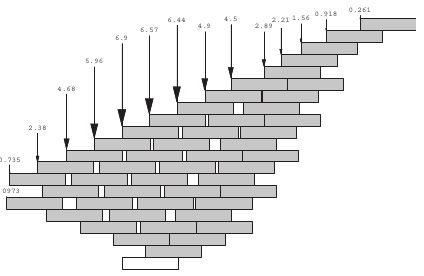
\includegraphics[scale=1]{pics/kirpich4}
\caption{Максимальный выступ для 100 кирпичей.}
\label{pic:kirpich4}
\end{figure}

\begin{figure}[htb!]
\centering
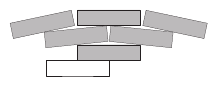
\includegraphics[scale=1]{pics/kirpich5}
\caption{Перевёрнутый треугольник разваливается начиная с трёх слоёв.}
\label{pic:kirpich5}
\end{figure}

Важный шаг сделали Майк Патерсон и Ури Звик в своей статье \cite{47} (она появилась в январе 2006 года, то есть написана до публикации статьи Холла).
Их статья доказывает, что Холл правильно вычислил возможный выступ хребетных стенок.
Однако они также показали, что хребетные стенки перестают быть оптимальными начиная с 20 кирпичей.
Что ещё поразительней, они построили стенку, дающую \emph{экспоненциально лучший} выступ, чем то, что считалось достижимым.

Наилучшая стенка из 20 кирпичей изображена на рис. \ref{pic:kirpich3};
она лишь незначительно обгоняет хребетную стенку Холла.
Однако, как видно из рис. \ref{pic:kirpich4},  при больших $n$ лучшие конфигурации перестают напоминать хребетные.
Стрелки в верхней части рис. \ref{pic:kirpich4} обозначают дополнительный вес некоторых не показанных кирпичей (из разрешённых 100), их положения определены неоднозначно.

На самом деле, для очень больших значений $n$ лучший выступ достигается для стенок, как будто вырезанных из обычной кирпичной кладки --- середина кирпича располагается ровно над стыком пары кирпичей ниже.
Тем не менее наиболее очевидные такие стенки разваливаются.
В книге Джаргодзки и Поттера \cite{38} (рекомендуется, несмотря на следующую ошибку) утверждалось, что устойчивы перевёрнутые треугольники (один кирпич внизу, затем два, затем три и так далее), но на самом деле они разваливаются, начиная с трёх слоёв (см. рис.~\ref{pic:kirpich5}).  

Стенки-ромбы (с добавлением кирпича на слой, до определённого момента, а потом назад до одного) устойчивы до семи слоёв, и на рис. \ref{pic:kirpich6} показано, что происходит далее.

\begin{figure}[htb!]
\centering
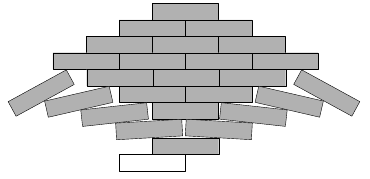
\includegraphics[scale=1]{pics/kirpich6}
\caption{Девятислойный ромб разваливается.}
\label{pic:kirpich6}
\end{figure}

Вместо этого Патерсон и Звик построили стены, форма которых напоминает параболы, показанные на рис. \ref{pic:kirpich7}.
Они строятся (и их устойчивость доказывается) рекурсивно, складывая то, что они называют $k$-плитами для последовательно возрастающих $k$.
Одна $k$-плита состоит из $2k + 1$ чередующихся слоёв, в каждом из которых по $k + 1$ и $k$ кирпичей.
Выступ, достигнутый параболической стеной из $n$ кирпичей, имеет порядок $\sqrt[3]{n}$ (кубический корень).%
\footnote{Мы говорим, что функция $f (n)$ (в нашем случае максимальный выступ для $n$ кирпичей) имеет порядок $g(n)$, если существуют положительные константы $c$ и $c'$ такие, что $c g(n) < f (n) < c' g(n)$.}

\begin{figure}[htb!]
\centering
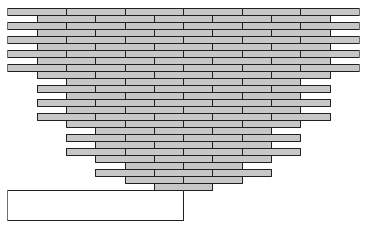
\includegraphics[scale=1]{pics/kirpich7}
\caption{Параболическая стена.}
\label{pic:kirpich7}
\end{figure}

А можно ли это улучшить?
Ромбы или перевёрнутые треугольники, если бы не разваливались, давали бы асимптотически лучший выступ, порядка $\sqrt{n}$ (квадратный корень).
Однако позднее Патерсон и Звик вместе с Ювалем Пересом, Миккелем Торупом и автором этих строк \cite{48} смогли показать, что порядок $n^{1/3}$ оптимален.

\begin{figure}[htb!]
\centering
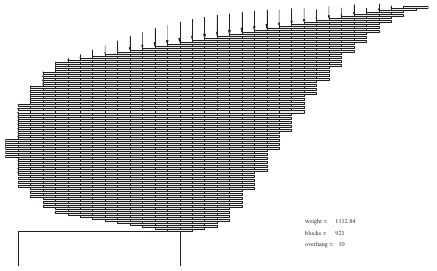
\includegraphics[scale=1]{pics/kirpich8}
\caption{Эта ламповидная форма стены, возможно, оптимальна.}
\label{pic:kirpich8}
\end{figure}

И всё же это не означает, что параболические кирпичные стены лучше всех.
Они дают выступ примерно $\tfrac3{16}n^{1/3}$, a другие могут дать $cn^{1/3}$ для большей константы $c$.
Патерсон и Звик считают, что лучшая форма для больших $n$ --- это форма «масляной лампы» на рис. \ref{pic:kirpich8}.

\begin{figure}[htb!]
\centering
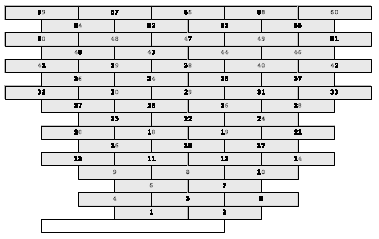
\includegraphics[scale=1]{pics/kirpich9}
\caption{Стенка, строящаяся кирпич за кирпичом.}
\label{pic:kirpich9}
\end{figure}

Параболическую кирпичную стену нельзя построить кирпич за кирпичом.
Причина в том, что, как и все устойчивые конфигурации, показанные выше, она находится на грани устойчивости.
Однако, немного изменив параболу, её всё же можно построить кирпич за кирпичом.
На рис. \ref{pic:kirpich9} показана такая модификация, все ещё обеспечивающая выступ порядка $n^{1/3}$.

Конечно же, стоит помнить, что настоящие кирпичи не идеально прямоугольны и ещё могут ломаться.
Поэтому не пытайтесь повторить это в домашних условиях!

%\begin{addedbytheeditors}
%\textbf{Редакторам.}
%Думаю, что здесь очень много ляпов. Пожалуйста, проверьте аккуратно.
%\end{addedbytheeditors}
